\documentclass[12pt]{article}
\usepackage[utf8]{inputenc}
\usepackage{amsmath}                         % math
\usepackage[letterpaper, portrait, margin=1in]{geometry}
\usepackage{amsfonts}                        % math symbols (ex: R^n)
\usepackage{amssymb}

\usepackage{graphicx}                        % imagens
\usepackage{hyperref}                        % hyperlink
\usepackage[usenames, dvipsnames]{color}
\usepackage{algpseudocode}
\usepackage{listings}
\lstdefinestyle{term}
{
    backgroundcolor=\color{black},
    basicstyle=\footnotesize\color{white}\ttfamily
}

\algrenewcommand\Return{\State \algorithmicreturn{} } % removes returns in the same line for code 
\usepackage{indentfirst}
\usepackage{enumitem}
\setlist[description]{leftmargin=\parindent,labelindent=\parindent}

% colors
\definecolor{title_color}{RGB}{60, 100, 200}
\definecolor{text_color}{RGB}{0, 0, 0}
\definecolor{section_color}{RGB}{25, 100, 75}
\definecolor{basic_dir}{RGB}{0, 255, 170}
\definecolor{svb}{RGB}{0, 50, 150}

% titles
\usepackage{titlesec}
\titleformat*{\section}{\LARGE\bfseries}

%\usepackage{helvet}
\renewcommand{\familydefault}{\sfdefault}

\title{420 Project}
\author{Gustavo Estrela de Matos}
\bigskip
\date{\today}

\begin{document}
\begin{titlepage}
\begin{center}
    \begin{flushleft}
        \textcolor{title_color} {
            \fontsize{2cm}{1em}\selectfont {Trying to break the RSA with Reversible Multiplier Circuits\\}
        }
    \end{flushleft}
  
    \begin{flushleft}{
        \textcolor{text_color} {
        \href{mailto:estrela.gustavo.matos@gmail.com}{Gustavo Estrela de Matos} 925003559\\}
    }
    \end{flushleft}
    \today
\end{center}
\end{titlepage}

\newpage
\section{The Problem}
RSA is an algorithm for data encryption used in many different security system and considered one of safest nowadays. This algorithm is based on the difficulty of the problem of factorizing the product of two large prime numbers, known as Integer Factorization Problem, which has no polynomial algorithm to solve (not considering that there are some polynomial algorithms for this problem in quantum computers).

\subsection{How to Break RSA Security}
The RSA algorithm has two different keys, a public and a private one. The private key is composed by two large prime numbers and the public key is composed by the product of these two primes, therefore, if we are able to factorize the public key we can get the private key,  which allows us to decrypt the message.

As mentioned before, the problem of factorizing integers is a hard problem and until today no one was able to give a polynomial algorithm to solve it. In this project we focus on creating a heuristic to find the prime factors that compose the public key of the RSA and crack the code.

The heuristic we are going to implement is based on the creation of a circuit that performs a reversible multiplier. This circuit is going to be composed of toffoli gates, which is a gate composed of control points and a controlled point. In a toffoli gate the open (closed) control point is satisfied if the input bit is 1 (0) and when all the control points are satisfied we toggle the controlled point. The circuit of a reversible multiplier is simply a set of toffoli gates.

\begin{figure}[h]
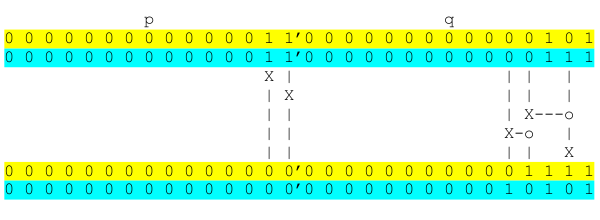
\includegraphics[scale=1.0]{MultiplierExample}
\caption{Example of a reversible Multiplier composed of toffoli gate. This multilpier is composed of five toffoli gates and it is capable of multiplying $3$ and $5$ (in yellow) and also $3$ and $7$ (in cyan). \emph{Figure available in http://courses.cse.tamu.edu/daugher/misc/PPP/homeworks/420-16spring-project.pdf}}
\end{figure}

\subsection{Goal of this Project}
In this project we intend to use search algorithms that we were exposed in class to solve the problem of finding the best multiplier possible, i.e the multiplier that correctly multiplies the greatest number of pairs of primes correctly. To do that we are going to use two search methods: genetic algorithms and local beam search. We are going to implement these two heuristics showing how we set up their parameters and also compare their efficiency.

\subsection{Restrictions and Limitations}
\label{restrictions}
It should be a know fact for the reader that the number of primes are infinite, therefore, as we explained before we do not intend to create a universal circuit capable of multiplying any pair of primes. The first limitation imposed in our algorithm is that toffoli gates and multilplier circuits only handle up to 30-bits number. Another limitation is that the input of a multiplier should be a 30-bits number $\overline{p}'\overline{q}$ where $\overline{p}$ and $\overline{q}$ are 15-bits representation of $p$ and $q$ respectively, and $p \leq q$, and this is what guarantee this circuit to be reversible (otherwise order changing would create a different solution).

In the development of this project we also had to restrict the number of primes that we were considering for multiplication, so then we would be able to see more effective results of both genetic algorithms and local beam search. Our limitation is that we are only considering the first fourty prime numbers, i.e primes between 2 and 173 (we can round up to 8 bit primes).

\section{Solving the Problem}
As mentioned before we implemented used two different approaches to solve this problem: genetic algorithms and local beam search. In this section we describe how we implemented the solution using these two different approaches and how we set up parameters for them based on experimentation.

\subsection{Solution Evaluation}
The first problem we faced in this project was to find a fast way to compute the fitness or the score of a solution. The first approach we used was to run the multiplier being tested to all possible combinations of 30-bits prime numbers. This approach showed to be too slow, which is not good because for both genetic algorithm and local beam search, the fitness function is called constantly.

To solve this problem we decided to add to our search method a parameter that stores the number of prime pairs (randomly chosen) that should be multiplied to calculate the fitness of a multiplier. This does not solve entirely the evaluation problem because now, since there are a lot of different pair of primes, it would be hard to distinguish a multiplier that works for one input from one that does not work for any input; that happens because the probability of choosing that one input is too small. Finally, we added a limit on the number of primes we consider for this problem, as we mentioned in the section \ref{restrictions}.

\subsubsection{Bit Entropy}
\label{bit-entropy}
Before explaining how we implemented both solutions present on this project we should understand the concept of entropy and how we can use it to guide our algorithms on the search for the best solution. In the context of this project we can define that the entropy of a bit is the inverse of the amount of information that this bit has, and by information we mean how certain are we that this bit needs to be toggled - or, complimentary, not toggled - from input to output. 

For instance, let's consider that the $i$-th bit has been correct for $90\%$ of the evaluations, then we can say that probably this bit will be correct for other pair of primes, and similarly, we can say that this bit will not be correct if it wasn't correct in the past evaluations. Knowing that, we can use this high informative bits to place our toffoli gates on bits that are normally incorrect and place the control points on bits that are normally correct.

\subsection{Genetic Algorithm}
The genetic algorithm approach consists of creating an initial set of multipliers, in this context called individuals, each one evaluated for some fitness function, and a sequence of iterations with crossovers and mutations. Each iteration generates a new generation of individuals that, in theory, should converge to a better fitting individual, which in this case is the individual that correctly multiplies the greates number of pairs of primes.

\subsubsection{Population Start}
Our first attempt to start the population with random multipliers, but this approach made necessary a lot of generations before finding a multiplier that scores. Trying to fix this, we implemented a multiplier constructor that receives two primes as a parameter and builds a multiplier that correctly multiplies the two arguments. That way we could start the population with multilpiers that we can guarantee that works well for at least one pair of primes.

\subsubsection{Crossover}
We tried two different approaches for crossing over two individuals $I_1$ and $I_2$, both of them considering the relative fitness:
\begin{itemize}
    \item{Random crossing: for every gate in $I_i$, add this gate with probability $RelativeFitness_1 (I_i)$}
    \item{Column random crossing: for every gate controlling the $j-$th bit of $I_i$, add all these gates to the child with probability $RelativeFitness_1 (I_i)$. If the sum of gates in the $j$-th column of both individuals is less than $5$, add all these gates to the child with probability $0.5$.}
    After some tests we concluded that the second approach was more effective than the first one.
\end{itemize}

\subsubsection{Mutation}
The mutation happens right after the crossover with probability of $0.5$, and it exploits the Bit Entropy as we defined in section \ref{bit-entropy}. The mutation only adds new gates to the child multiplier, placing the gate on a bit that is frequently incorrect with up to $6$ (random) control points placed in frequently correct bits. We also tried totally random gates, but that haven't shown to be effective.

\subsubsection{Fitness Function}
The fitness function used in the genetic algorithm is simlpy the number of correct multiplications seen when evaluated the individual.

\subsubsection{Parameter Settings}
The genetic algorithm has several parameters including: population size, number of primes used to evaluate and probability of mutation. The most important parameter to set up between those is the number of primes to evaluate, because this number has big impact in the time needed to create a new child in a crossover, and, since we want the algorithm to have as many iterations as possible (so we can get evolved individuals) it is important to choose this parameter in a way that the evaluation of a new child happens fast.


\subsection{Local Beam Search}
The Local Beam Search algorithm is similar to a random walk with $k$ different nodes and a function that we are going to call fitness function as we did for the genetic algorithm. The algorithm starts with a population of $k$ empty multipliers, i.e there are no gates in the multipliers and for each step we do the following:
\begin{itemize}
\item{Generate a number of successors for every $k$ node;}
\item{Choose the best $k$ nodes between successors and current nodes all and repeat.}
\end{itemize}
\subsubsection{Fitness Function}
With a few tests we realized that when we look into a node successors, many of them have the same score when considering the number of correct multiplications. Also, if we consider the number of correct bits we end up guiding the algorithm to solutions that, on average, has a good number of correct bits but not necessarily multiplies two primes correctly. Therefore, we decided to use a fitness function that has both information:
\begin{center}
    $FitnessFunction_2 (N_i) = 60 * FitnessFunction_1 (N_i) + BitScore (N_i)$
\end{center}

\subsubsection{Choosing Next Step}
Every iteration we open a certain number (set as a parameter) of successors and to do that we copy all gates from the current node and we generate the new multiplier by either:
\begin{itemize}
    \item{Adding a new gate with probability $3/5$;}
    \item{Adding a new control point with probability $1/5$;}
    \item{Removing a gate with probability $1/5$}
\end{itemize}

To accomplish these actions we use again the Bit Entropy concept we presented in section \ref{bit-entropy} in a similar way as we did for the genetic algorithm. When we add a gate we should choose as the control to be on a bit that is frequently wrong and when adding a control point we should choose a bit that is frequently correct.

\subsection{Parameter Setting}
The Local Beam Search algorithm we implemented have some parameters we can set up, including the same parameter of number of primes to evaluate as we had for the genetic algorithm. We should note that the local beam search generates way more multipliers in an iteration, therefore, there are more calls to the evaluation function and we should set these evaluation to test less prime numbers than we did for the genetic algorithm.

\section{Results}
\subsection{Sample Run}
\begin{figure}[h]
    \centerline{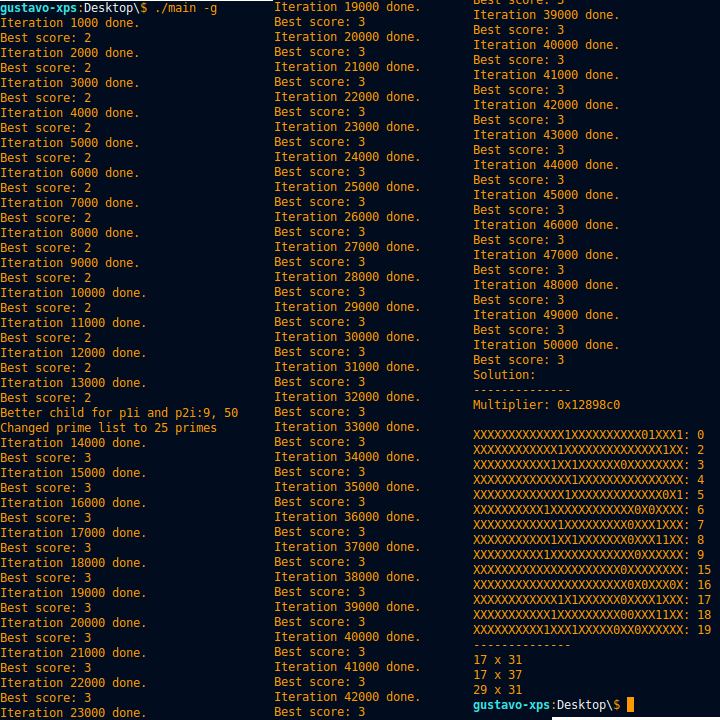
\includegraphics[scale=.5]{GASampleRun}}
\caption{Sample run of the genetic algorithm}
\end{figure}
\begin{figure}[h]
    \centerline{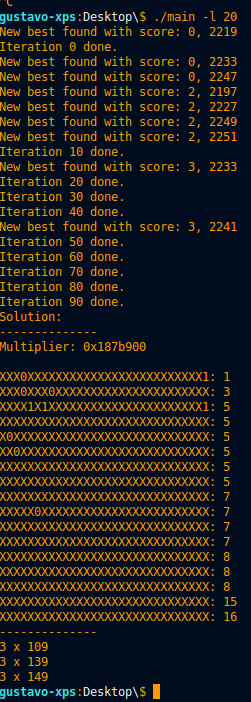
\includegraphics[scale=.5]{LBSampleRun}}
\caption{Sample run of the local beam search algorithm}
\end{figure}

\subsection{Analysis}
What we could observe from both algorithms was that they had a reasonable learning curve, but at some point they got stuck and they wouldn't find other multipliers with better scores. We believe that this learning limit happened because of the limit we imposed to the evaluate function for both, genetic algorithm and local beam search, when we restricted the set of primes to only the first 40 primes.

To compare both algorithms and also to help parameter tunning we print in a file, for both algorithms, the maximum score (number of correct multiplications) and maximum bitscore (number of correct bits) of that iteration. To visualize this data we created a \emph{gnuplot} script that creates a graph of this data and saves it in a \emph{.png} file. 

\begin{figure}[h]
    \centerline{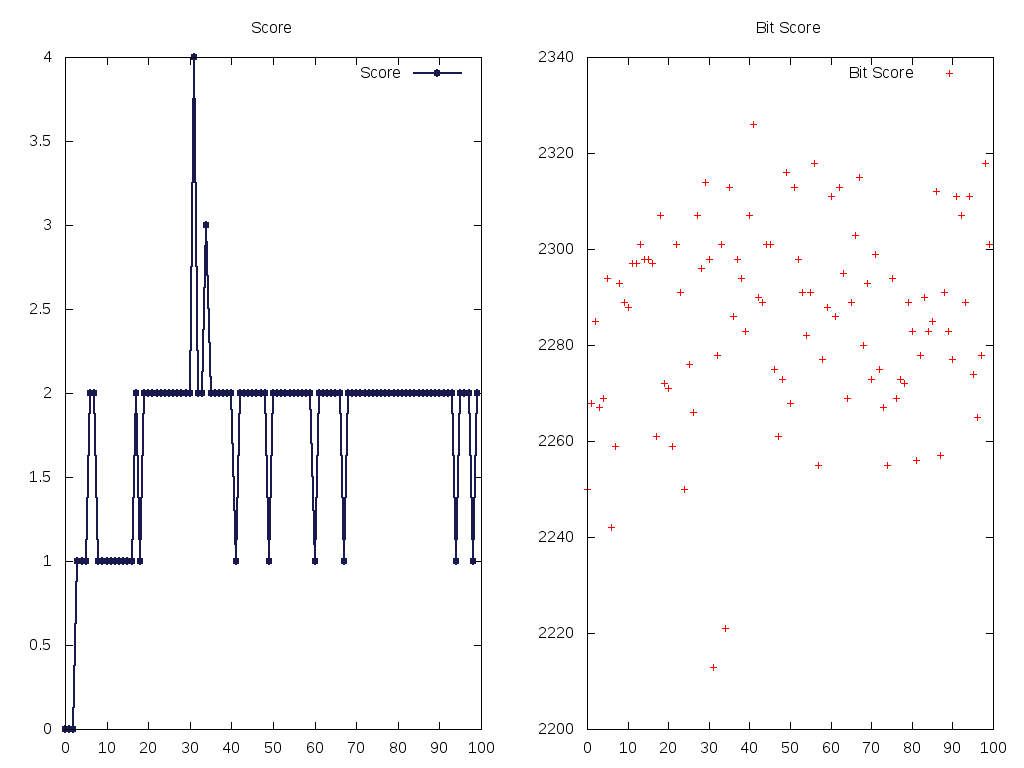
\includegraphics[scale=.5]{LBAnalysis}}
\caption{Score per iteration of the local beam search algorithm with 20 different beams.}
\end{figure}

\begin{figure}[h]
    \centerline{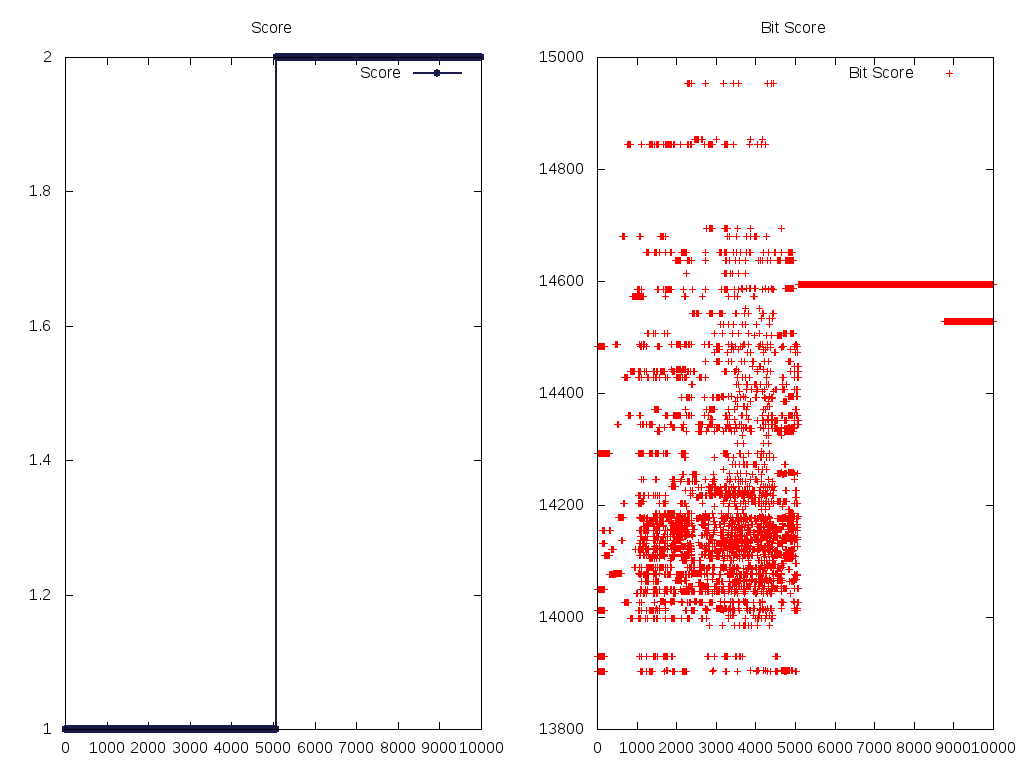
\includegraphics[scale=.5]{GAAnalysis}}
\caption{Score per iteration of the genetic algorithm. We can see that after finding a better solution, the algorithm has a very constant bit score, and that happens because this algorithm only considers Score when evaluating its solutions, therefore when the solution does not change the bit score tend to be the same.}
\end{figure}

We can see in the graphics is that the local beam search algorithm was more successful than the genetic algorithm because, even starting with the advantage of having working multipliers, the genetic algorithm, in general, couldn't find as many solutions as the local beam algorithm could. 

We could say that the strategy of genetic algorithm was not better than the local beam because it's not really easy to create a crossover and mutation that, at the same time has a random factor enough for walking on the search space and does not destroy the solution (does not make it worse). The local beam search, differently, we don't take big random steps, therefore we don't risk our current solutions of giving big steps to worse solutions every iteration.


\section{Conclusion}
We conclude that, even though our algorithms showed some progress in their learning curve, we did not achieve the what the title of this project suggests. To see that, first we should remember that RSA cryptography uses numbers way bigger than 30-bit numbers, and also, we restricted our program to consider only the 40 first primes, therefore, our results are not even close to break a real RSA code.

\subsection{Lessons Learnt}
Even though we did not get close to break the RSA code, the process of creating the algorithms implemented in this projects gave us more knowledge in computer science that can be used to solve different problems, or even try another approach to get closer to break the RSA code.

In this project we learnt how the RSA cryptography is based on the simple, but very hard, problem of factorizing big numbers. We also learned how it is possible to create a reversible circuit and therefore solve the factorization problem with a "simpler" problem of multiplying two numbers.

The implementation of both algorithms made us face more than the usual issues we face when implementing something in computer science, which is normally just technical issues such as segmentation faults. Since we had the freedom of choosing how we were going to solve the problem, we had to elaborate, experiment and analyse approaches. 

\subsection{Future Research}
Since we did not have a lot of time to work on this project, there are some parts of it that could be explored with a little more rresearch. The first thing we could work on this project to make it better is to run more tests varying all the parameters we used in both genetic algorithm and local beam search. 

For instance, we could research and improve in this project changing the evaluation of the fitness function. It was clear for us that considering only \emph{Score} and \emph{Bit Score} was not a very good fitness function, but we did not try a lot of different combinations of fitness functions that consider both \emph{Score}, \emph{Bit Score} and other parameters.

We could also research on how to increase the set of primes being considered with the growth of the fitness function. There is a trade-off on the number of primes we are considering which is the following: if we consider a large set of primes, it is harder for the algorithm to be guided to a solution; but if the set is too small the algorithm can get stuck or too restricted to that small set.

\section{Running Instructions}
All algorithms were coded in c++14 and to run the program you should:
\begin{itemize}
    \item{Run \emph{make} to compile}
    \item{Run \emph{./main -l k or -g} to run the code. Use \emph{-l k} to run local beam search with k beams and \emph{-g} for genetic algorithm.}
    \item{Run \emph{gnuplot ./plot\_script.gp} to generate score plot; the output is a \emph{.png} file.}
\end{itemize}
\end{document}
